\documentclass{article}
\usepackage[utf8]{inputenc}
\usepackage[spanish.mexico]{babel}
\usepackage[american voltages, american currents,siunitx]{circuitikz}

%Plotting

\usepackage{pgfplots}
\pgfplotsset{width=10cm,compat=1.9} 
 \usepgfplotslibrary{external}
\tikzexternalize 

%Diagrama de bloques

\usetikzlibrary{shapes.geometric, arrows}

\tikzstyle{startstop} = [rectangle, rounded corners, minimum width=3cm, minimum height=1cm,text centered, draw=black, fill=red!30]
\tikzstyle{io} = [trapezium, trapezium left angle=70, trapezium right angle=110, minimum width=3cm, minimum height=1cm, text centered, draw=black, fill=blue!30]
\tikzstyle{process} = [rectangle, minimum width=3cm, minimum height=1cm, text centered, draw=black, fill=orange!30]
\tikzstyle{decision} = [diamond, minimum width=3cm, minimum height=1cm, text centered, draw=black, fill=green!30]


\tikzstyle{arrow} = [thick,->,>=stealth]
%###MIO###
\tikzstyle{point} = [circle,(0.5cm),minimum with=1cm,draw=black,fill=black!50]




\title{Previo 5: Ruido}
\author{Pablo Vivar Colina\\
Grupo 13
}
%\date{Septiembre 2017}

\usepackage{natbib}
\usepackage{graphicx}

\begin{document}

\maketitle

\section{Ruido}

La mayoría de las aplicaciones se tiene o considera al ruido r como aditivo, esto es para la señal enviada $s$ se tiene que:\citep{Capitulo1SC}\\

\begin{equation}
    x_r=s+r
\end{equation}

Donde $x_r$ es la señal recibida.\citep{Capitulo1SC}\\

El ruido natural tiende a ser gaussiano, esto es, su densidad es:\citep{Capitulo1SC}

\begin{equation}
    p(n)=\frac{1}{\sqrt{2 \pi \sigma_n}} e^{-\frac{(m-n_m)^2}{2 \sigma_n^2}}
\end{equation}

\begin{figure}[h!]
    \centering
    
   
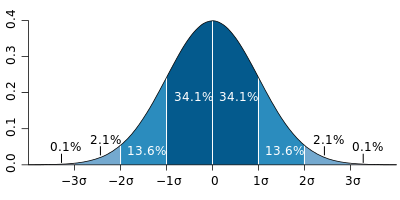
\includegraphics[width=0.6\textwidth]{Imagenes/Standard_deviation_diagram.png}
\caption{ La distribución Normal suele conocerse como la "campana de Gauss".}
    \label{fig:distNorm}
 
\end{figure}


Refiriéndonos a la distribución normal, la cual podemos apreciar en la figura \ref{fig:distNorm} tenemos que:\citep{DistribucionNormal}\\

\begin{itemize}
    \item $\sigma^2$ es la varianza
    \item $n_m$ es la moda
\end{itemize}


El ruido más común es blanco y se define como aquel de densidad de potencia constante.\citep{Capitulo1SC}\\

\begin{equation}
    G_n(f)=\frac{N_0}{2}
\end{equation}

entonces:\\


\begin{equation}
    R_n(\tau)=\frac{N_0}{2} \delta (\tau)
\end{equation}

El ruido térmico es blanco, aditivo y gaussiano, como este ruido esta presente en todos los sistemas de comunicaciones, se utilizan sus características para modelar ruido en comunicaciones.\citep{Capitulo1SC}



%####AQUI VAMOS###





\bibliographystyle{plain}
\bibliography{Referencias.bib}


\end{document}